%*************************************************************
% Master Project                                             *
% Ing. Minerva Gabriela Vargas Gleason                       *
% IAI - Institute of Artificial Intelligence                 *
% Universit�t Bremen                                         *
%                                                            *
% pdfLaTex                                                   *
% Editor: TeXnicCenter                                       *
%*************************************************************


\chapter{Discussion}

%The main results achieved during the development of this project were:
%
%\begin{itemize}
%	\item Updating URDF model of boxy, including virtual links used for the trayectory planning of the Kinect.
%	\vspace{-5pt}
%	\item Solving compatibility problems between MoveIt! and the STLs generated by inventor.
%	\vspace{-5pt}
%	\item Generating collision-free paths for the UR3 robot.
%	\vspace{-5pt}
%	\item Correctly orienting the Kinect such that Boxy looks at the objects it will interact with.
%	\vspace{-5pt}
%	\item Configuring Boxy for trajectory planning with MoveIt!
%	\vspace{-5pt}
%	\item Successful implementation during the RoboHow demo.
%	\vspace{-5pt}
%	\item Target position can be specified as a pose or in joint values.
%\end{itemize}
%
%\begin{figure}[H]
%	\centering
%	\begin{subfigure}[][Simulation]
%		{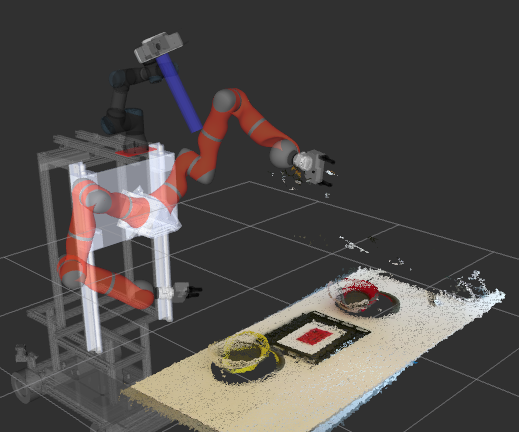
\includegraphics[width=0.3\linewidth]{boxy/results2.png}}
%	\end{subfigure}
%	\begin{subfigure}[][Real Robot]
%		{\label{subfig:goal}
%		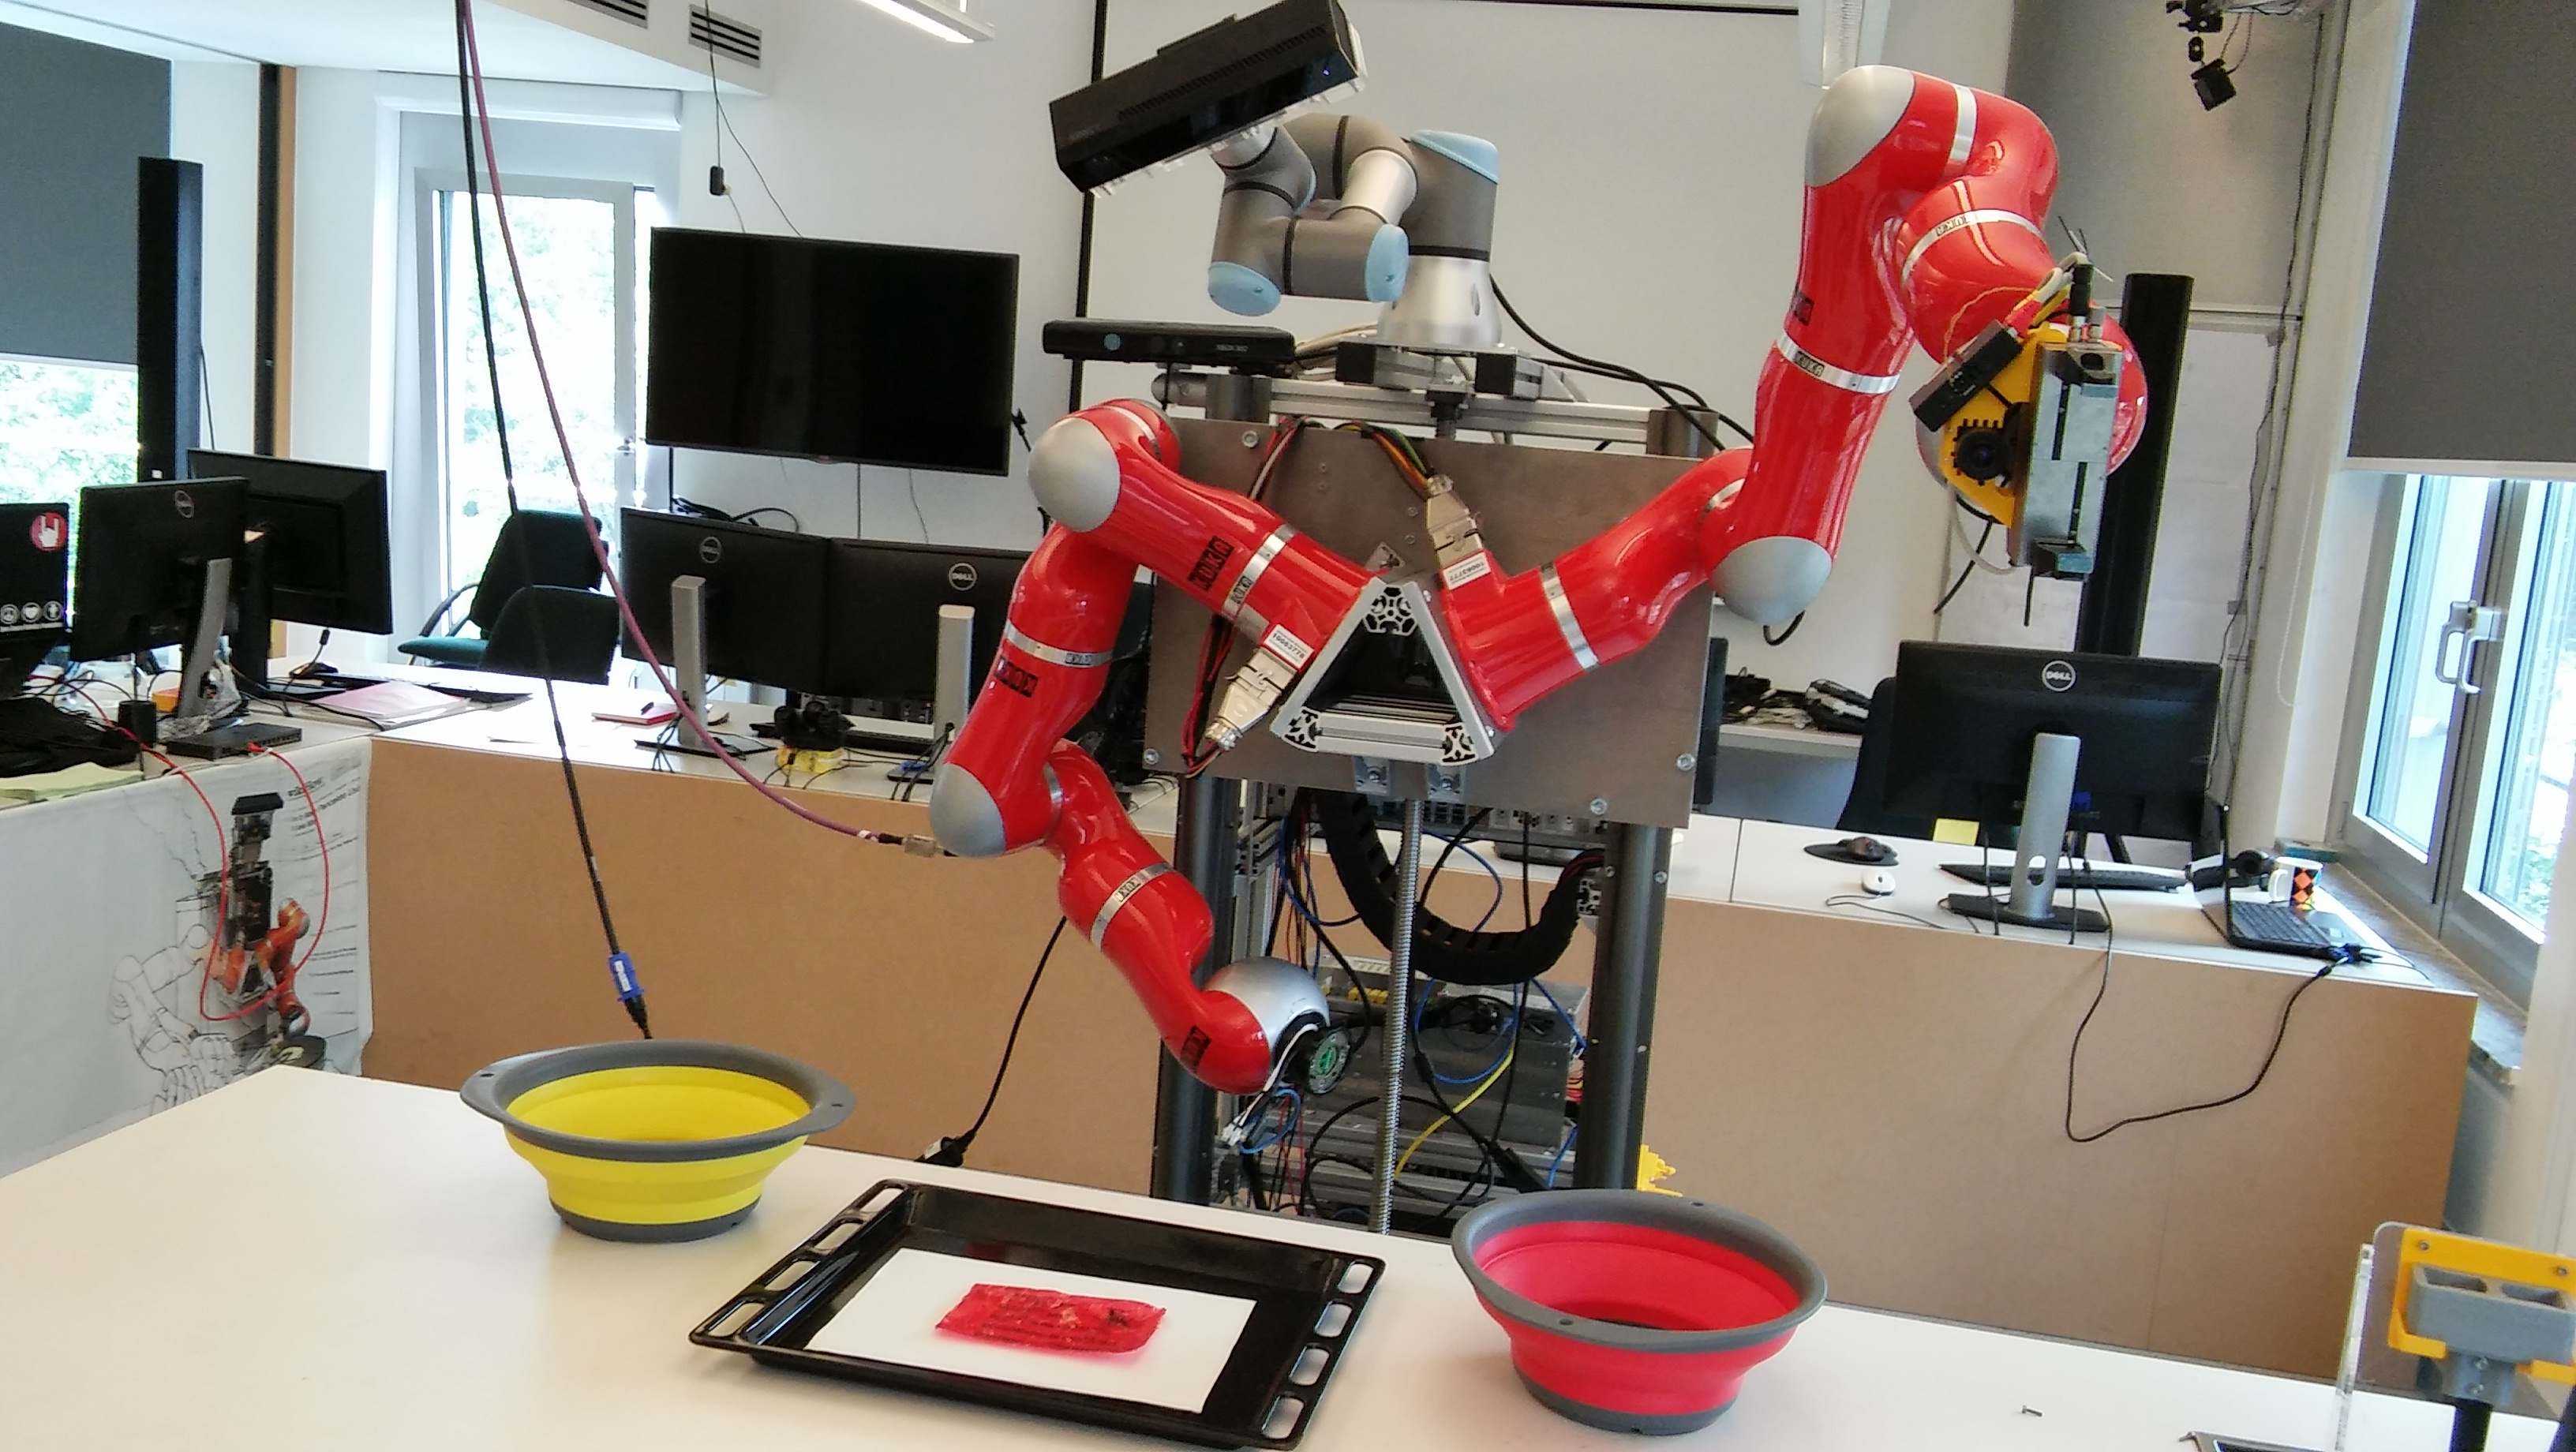
\includegraphics[width=0.45\linewidth]{boxy/Boxy3.jpg}}
%	\end{subfigure}
%	\vspace{-12pt}
%	\caption{Microsoft Kinect 2 correctly oriented after code execution}
%	\vspace{-15pt}
%	\label{fig:example}
%\end{figure}
%\vspace{-8pt}
%Figure \ref{fig:example} shows an example of a trajectory executed on the robot and visualized on RViz, where the Microsoft Kinect 2 reached an orientation where Boxy can see the objects it will interact with.
%
%All the GitHub repositories required to execute this code are found in appendix \ref{A2}.